\chapter{Log-Log Plots}
\thispagestyle{fancy}
\fancyhead[RE,LO]{Technical Document \thechapter}

\section{Powers \& Exponents}
In understanding how one variable depends on another, we introduced the idea of \emph{functional dependence}.
This helps us understand not just that one variable depends on another, but how it depends on the other.
This is especially important in complex situations such as biology where many variables can be involved and "which one dominates" matters.

\subsection*{Powers}
Some of the most useful and convenient functional dependencies that we will encounter are \textbf{power laws}.
This means that the variable we choose to be dependent depends on the variable we choose to be independent by some power of that variable.
Thus
\[ y = f(x) = x^{N} = x \text{ multiplied by itself } N \text{ times} \]
says that ``\emph{y goes like x raised to the Nth power}''.

\subsection*{Exponentials}
We know that a quadratic function rises faster than a linear one (eventually) and a cubic rises faster than a quadratic.
But there is an extremely useful function that eventually rises faster than any power.
This is the exponential function.
In this case, the variable is not raised to a power - the variable itself is in the power that some constant is raised to.
So as the variable gets bigger and bigger, the power the constant is raised to gets bigger and bigger.
\par
We write
\[ y = e^{x} \text{.} \]
Now e could be any constant, but we typically take it as a special transcendental number (that means it's decimal representation never stops and never repeats): $e = 2.712...$
This particular choice is because when we make this choice, the function ex is its own derivative.
That is, if we write $y = e^{x}$, then
\[ \frac{dy}{dx} = y \text{.} \]
[Note that a power law is not referred to as an ``exponential dependence'' even though the variable ``has an exponent''.
That terminology is reserved for the case when the variable is in the exponent.]
\par
In case you wondered how in the world a calculator figures out what ``$e$'' to the something is, the following result allows you to calculate the value of $e$ raised to some number -- eventually.
\[ e = 1 + x + \frac{x^{2}}{2} + \frac{x^{3}}{6} + \frac{x^{4}}{24}+... \]
You can see how this goes on - and it goes on forever.
But for any fixed x you are calculating for, the denominators go up faster than powers do and so eventually start making the terms smaller and smaller so they can be dropped.
\par 
While this looks really messy and we're not going to use it, looking at it does give us two interesting messages.
\begin{enumerate}
\item \textbf{It explains why the exponential function is its own derivative.} If you take the derivative of the power series representation of the exponential, something interesting happens. The first term vanishes, the derivative of the linear term becomes the old first term (1), the derivative of the third (quadratic) term becomes the old second (linear) term, etc.  So the derivative of each term becomes the previous term in the original series.  We wind up getting the same thing back that we started with.  This also shows us why the denominators have the structure they do. [And with a little fancy mathematical footwork, we can show that the exponential is the only function that is its own derivative.]
\item \textbf{It shows that we can only take exponentials of pure numbers.} Since we know that you can't add a length and an area - or any quantity that has units to its square - the power series only makes sense if ``x''  is a pure number.  You can't take an exponential of a quantity that has units.  Whenever in science we have an exponential, it will always be the ratio of two quantities with the same units - typically a variable and a scale for that variable.  (Like a time and a rate constant.)
\end{enumerate}

\subsection*{Logarithms}
The exponential function does the interesting thing of converting sums into products.
If $R = e^{a}$ and $S = e^{b}$ then $R \cdot S = e^{a+b}$.
So if $f(x) = e^{x}$ then we have
\[ f(x_{1})f(x_{2}) = f(x_{1} + x_{2}). \]
Since multiplying is harder than adding, it's sometimes useful to go backwards from the exponential function. 
Taking the exponential of $x$ and setting $y = e^{x}$, if we are given $x$ we can use our calculator (or series) to find $y$.
But what if we are given $y$ and want to find $x$?
The answer to that is called the \emph{natural logarithm} of $y$.
So that would give us the equation:
\[ y = e^{ln(y)} \]
This shows that the natural log ($ln$) is the inverse function of the exponential.
If we first take the natural log and then exponentiate it, we get back what we started with.
It works the other way too:
\[ x = ln(e^{x}) \]
If we exponentiate first and then take the natural log, we get back what we started with.
So the natural log function ($ln$) undoes the exponential function and vice versa.
We will see in the follow-ons that logarithms and exponentials are very useful in analyzing data and seeing whether something behaves like a power law. 

\section{Log-Log Plots}
When we have a complicated function it is sometimes useful to approximate it by a simple power law.
One way to see how to do this is to use a \emph{log-log plot}.
That is, instead of just plotting the variables themselves, we plot the logarithm of the variables.
Let's see how this works.
Suppose we have a power law function $y = x^{N}$.
If we plot this, we get a curve like shown in figure \ref{fig:lin-log}.
The more powers we have, the faster it rises (and the odd powers are negative for negative values of x.)
But if we take the logarithm of both sides of that equation, $y = x^{N}$,we get
\[ log(y)=N \cdot log(x) \] 
If we now take as new variables $Y = log(y)$ and $X = log(x)$, then our new equation is just $Y = N \cdot X$.
This is the graph of a straight line and the slope is proportional to the power.
If we plot this we get the figure at the right.
All the power laws are straight lines with increasing slope as the powers go up.
So if we have some complicated function that can be approximated by a power law, we can easily see that this is the case by plotting the logarithms of the variables. 
If we get a straight line a power law works. 
(We have only plotted positive values of x and y in the log-log plot since the log of a negative number is not a real number.)
Note that this works for negative powers too. 

\begin{figure}[h]
	\centering
	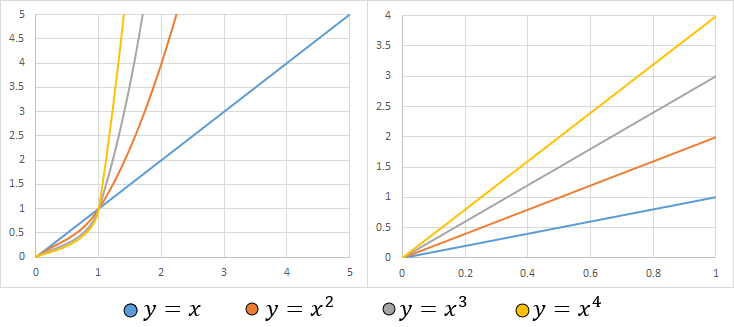
\includegraphics[width=0.7\linewidth]{linVSlog.png}
	\caption{Comparison of linear vs. log-log graphs.}
	\label{fig:lin-log}
\end{figure}

\section{Log-Log Plots in Science}
Log-Log plots have many uses in science.
They are especially helpful for differentiating between different forms of \emph{functional dependency}.
What is functional dependency? 
Functional dependency tells us how one quantity varies when another is adjusted. 
Example: for purely random motion, the diffusion of an object in 2-D space has a functional dependence like $\langle r^{2} \rangle = 4 D \Delta t$. 
As you saw in lab, the viscosity and temperature of the fluid medium surrounding the object and the size of the object can affect the value of the diffusion constant, D, and thus the linear slope of the $\langle r^{2} \rangle$ vs.\ $\Delta t$ plot (where the slope is related to D). 
A $log(\langle r^{2} \rangle)$ vs.\ $log(\Delta t)$ plot of this functional dependency would be a line with a slope of 1 — regardless of the value of the diffusion constant, D! 
If we are not learning the diffusion constant D from this log-log plot, what does the slope of 1 tell us?
\par 
It turns out that the slope of $log(\langle r^{2} \rangle)$ vs.\ $log(\Delta t)$ tells us about what type of motion we are observing! 
Most motion will not be linear in an $\langle r^{2} \rangle$ vs.\ $\Delta t$ plot. 
There are other functional dependencies that can exist governing the relationship between $\langle r^{2} \rangle$ and $\Delta t$. 
For directed motion at constant velocity, $\langle r^{2} \rangle$ changes as $(\Delta t)^{2}$ and so the $\langle r^{2} \rangle$ vs.\ $\Delta t$ plot would be quadratic. 
But a $log(\langle r^{2} \rangle)$ vs.\ $log(\Delta t)$ plot of this motion is still linear, with a slope of 2. 
For directed motion under uniform acceleration from rest, the distance traveled is $r = \frac{1}{2} a \Delta t^{2}$, so $\langle r^{2} \rangle$ changes linearly with $(\Delta t)^{4}$ — thus a $log(\langle r^{2} \rangle)$ vs.\ $log(\Delta t)$ plot of this motion has a slope of 4!
\par 
Other motion in cells is confined, e.g. molecules that are caged by a surrounding scaffolding of actin, or molecules on the membrane that are confined to a ``lipid raft'' or patch of membrane that has some functional activity. 
For such caged motion, $\langle r^{2} \rangle$ does not quite increase linearly with $\Delta t$ — the distance moved gets smaller than we would expect for random motion as we get to larger and larger distances — thus a $log(\langle r^{2} \rangle)$ vs.\ $log(\Delta t)$ plot of this motion has a slope of less than 1.
 \par
For real biological systems, the motion is often a combination of random and directed motion — and thus a $log(\langle r^{2} \rangle)$ vs.\ $log(\Delta t)$ plot of this motion has a slope between 1 and 2. 
The dominant functional dependency (the one that determines the type of motion we observe) can also depend on the time scale at which we observe the motion.
\par
This is all very interesting, but how is it helpful to us?
In biology, almost all motion can look quite random, but that apparently random motion can hide other processes that may look similar to random motion — in particular, caged motion:

\begin{figure}[h!]
	\centering
	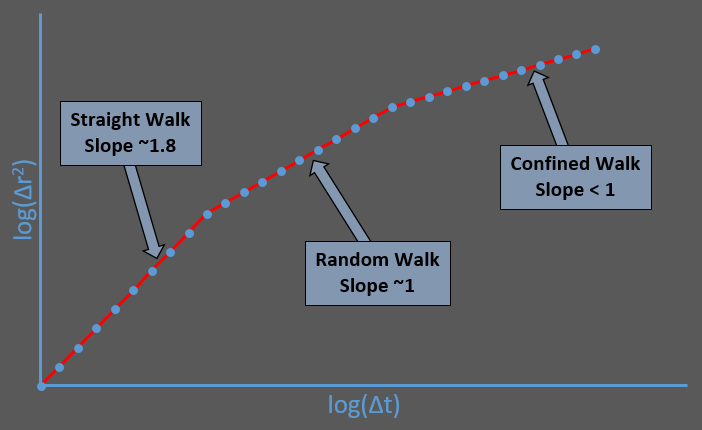
\includegraphics[width=0.6\linewidth]{log_diff.png}
	\caption{Example investigation of live motion analysis using log-log plots.}
	\label{fig:log-diff}
\end{figure}

\begin{itemize}
\item In ecology, tracking data from tagged animals can be analyzed to find the roaming grounds of an animal.
However, to distinguish random motion from the confined area to which an animal intentionally returns, we cannot simply look at the tracks by eye.
A log-log plot can help us find the distances at which the motion gets confined; helping us determine the size of roaming grounds and how often roaming grounds are changed.
In addition, on shorter timescales the motion will look directed since animals are able to move straight (at least over short distances)!
\item On much smaller scales, within cells, the tracking data from individual molecules on a cell membrane have helped develop the theory of ``lipid rafts''. Such rafts are patches of membrane that float on the overall cell membrane. Within the raft sit a number of functional molecules that appear to operate together, taking advantage of their closeness to each other within a raft to enhance signals. The significance of lipid rafts in biology is still under investigation and log-log plots are a key tool to distinguish randomness from caged motion!
\end{itemize}
%
Below is a chart to help summarize the broad categories of functional dependency and their effects on the slope of the $log(\langle r^{2} \rangle)$ vs.\ $log(\Delta t)$ plots.

\begin{table}[h!]
	\centering
	\begin{tabular}{|l|c|}
	\hline 
	Type of motion & Slope of the $log(\langle r^{2} \rangle)$ vs.\ $log(\Delta t)$ plot \\ 
	\hline 
	Confined & $s < 1$ \\ 
	\hline 
	Random & $s = 1$ \\ 
	\hline 
	Biological & $1 < s < 2$ \\ 
	\hline 
	Directed & $s = 2$ \\ 
	\hline 
	Accelerated & $s > 2$ \\ 
	\hline 
	\end{tabular} 
	\caption{The effect of movement type on a log-log plot.}
	\label{tab:logPlt}
\end{table}
These types of plots can also help us model a new phenomenon. 
Imagine a situation in which you wish to develop a model of how a biological or chemical process spreads in space with increasing time. 
Knowing the functional dependency between $\langle r^{2} \rangle$ and $\Delta t$ can help you build a model or help you choose between competing models. 
Once we understand the model better, we can make predictions about what will happen when we make changes to the system. 
In order to help us with our modeling, we take data on the motion and make a plot of $log(\langle r^{2} \rangle)$ vs.\ $log(\Delta t)$. 
The slope of this plot helps us make decisions about what models to propose or what models to eliminate. 
It also tells us which functional dependency dominates at which time scales — it tells us when a type of motion is the most important and when we can ignore the effects of other types of motion.
\par
(Note that log-log plots help with functional dependencies more generally. 
In chemistry, you may need to plot the log of a molecule's solubility vs.\ the pH.
Since the pH is the log of the number of free hydrogen ions, this is again a log-log plot in disguise! 
Then the slope can tell you how many charges an atom or molecule has in solution.)